% So we make this "beamer" rather than document!

\documentclass[11pt]{beamer}
% For handout add ,handout after 11pt

\usetheme[sectionpage=none,numbering=none]{metropolis}           % Use metropolis theme
	% To do printouts, add ", handout"  after aspectratio.
\usepackage{booktabs}
\usepackage{graphicx}
\usepackage{color}
\usepackage{ulem}
\title{Putting It All Together}
\author{\small Nick Eubank}
\date{\vspace*{.3in} \date}


% This is the beginning of a real document!
\begin{document}


\begin{frame}[c]
\maketitle
\end{frame}

\begin{frame}[c]{}
  \pause Data Science is the art of \alert{answering questions} about the world using \alert{quantitative data.} 
\end{frame}

\begin{frame}[c]{}
 \begin{enumerate}
   \pause \item Move from \alert{problems to questions}
   \pause \item Recognize the \alert{type} of question you are asking 
   \pause \item Understand how to choose the \alert{right tool} to answer the question you are asking
 \end{enumerate}
\end{frame}

\begin{frame}[c]{Types of Questions}
  \begin{enumerate}
    \pause \item Descriptive Questions \\
    {\color{gray} Identifying patterns in the world}
    \pause \item Causal Questions \\
    {\color{gray} Understanding the \emph{effects} of manipulations}
    \pause \item Predictive Questions \\
    {\color{gray} Making out-of-sample predictions}
  \end{enumerate}
\end{frame}


\begin{frame}[c]{Types of Questions}
  \begin{enumerate}
    \item \alert{Descriptive Questions} \\
    {\color{gray} Identifying Patterns in the World}
    {\color{gray} \item Causal Questions \\
    {\color{gray} Understanding the \emph{effects} of manipulations}
    \item Predictive Questions \\
    {\color{gray} Making out-of-sample predictions} }
  \end{enumerate}
\end{frame}


\begin{frame}[c]{Purpose of Descriptive Questions}
\pause Help identify areas for further investigation / prioritization 
\end{frame}
  

\begin{frame}[c]{Descriptive Questions}
\pause When answering a descriptive question, you are always doing \alert{dimensionality reduction}.
\begin{itemize}
  \pause \item Formally: PCA
  \pause \item Informally: picking what variables to plot, summary statistics to include, etc. 
\end{itemize}
\end{frame}

\begin{frame}[c]{Descriptive Questions}
  When answering a descriptive question, you are always doing \alert{dimensionality reduction}. \pause And so you will necessarily be \alert{discarding information}, and so it is \alert{your responsibility to:}
  \begin{itemize}
    \pause \item Ensure what you present faithfully represents the patterns in the underlying data. 
    \pause \item You make sure to look for ethically-salient patterns (differences by race, ethnicity, gender, etc.)
  \end{itemize}
  \end{frame}
  

\begin{frame}[c]{}
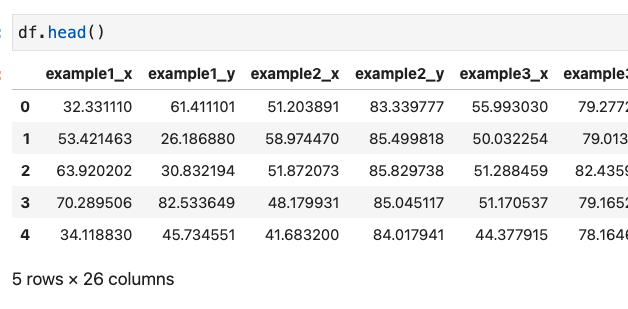
\includegraphics[width=\textwidth]{datasaurus_1.png}
\end{frame}

\begin{frame}[c]{}
  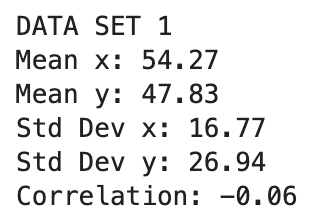
\includegraphics[width=0.5\textwidth]{datasaurus_sum_1.png}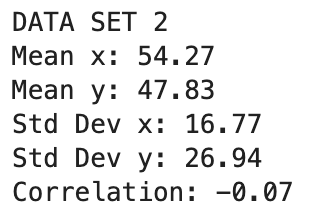
\includegraphics[width=0.5\textwidth]{datasaurus_sum_2.png}\\
  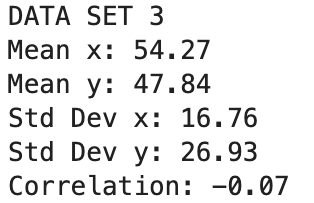
\includegraphics[width=0.5\textwidth]{datasaurus_sum_3.png}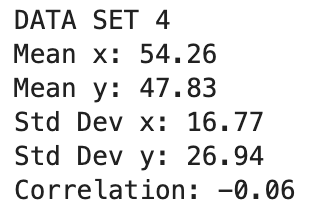
\includegraphics[width=0.5\textwidth]{datasaurus_sum_4.png}
\end{frame}

\begin{frame}[c]{}
  \pause 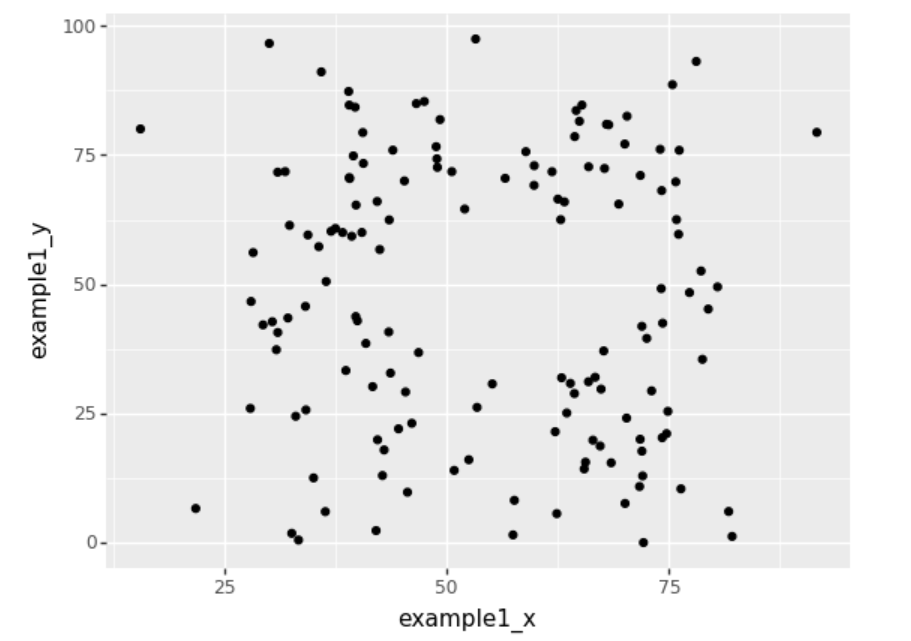
\includegraphics[width=\textwidth]{datasaurus_plot_1.png}
\end{frame}

\begin{frame}[c]{}
  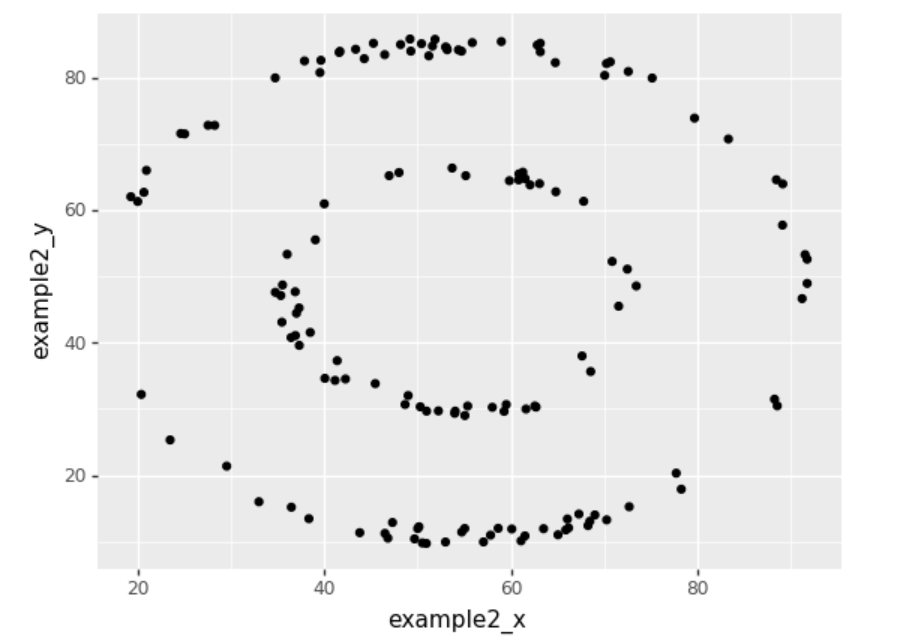
\includegraphics[width=\textwidth]{datasaurus_plot_2.png}
\end{frame}

\begin{frame}[c]{}
  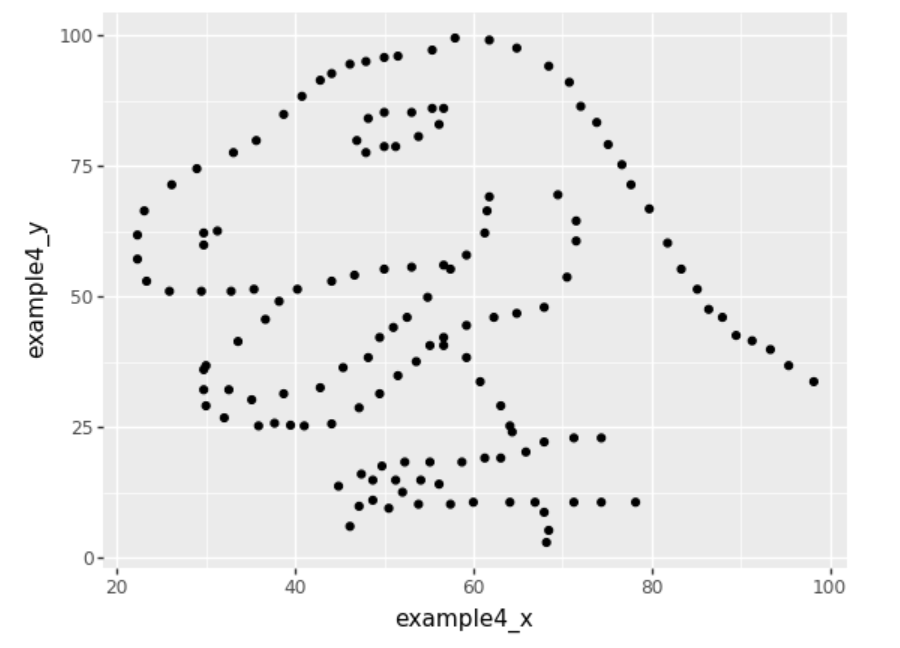
\includegraphics[width=\textwidth]{datasaurus_plot_3.png}
\end{frame}


\begin{frame}[c]{}
These all had the same means, standard deviations, and correlations. \\ 
\vspace{0.5cm}
\pause But if you had only reported those summary statistics, you would \alert{not have been faithfully representing the data}.
\end{frame}

\begin{frame}[c]{Types of Questions}
  \begin{enumerate}
    {\color{gray} \item {Descriptive Questions} \\
    {\color{gray} Identifying Patterns in the World} }
    \item \alert{Causal Questions} \\
    {\color{gray} Understanding the \emph{effects} of manipulations}
    {\color{gray} \item Predictive Questions \\
    {\color{gray} Making out-of-sample predictions} }
  \end{enumerate}
\end{frame}

\begin{frame}[c]{Purpose of Causal Questions}
  \pause Causality is about predicting the consequences of \alert{manipulations}.  \\
\pause $\rightarrow$ Generally asked in anticipation of undertaking some action. 
  \end{frame}
  
\begin{frame}[c]{Causal Inference}
  \pause Causal inference is \alert{hard}.
\end{frame}

\begin{frame}[c]{Causal Inference}
  Causal inference is hard because of the \alert{Fundamental Problem of Causal Inference:} \\
  \pause We say that ``X caused Y'' if:
  \begin{enumerate}
    \pause \item When X is present, we see Y
    \pause \item When X is not present, we don't see Y
  \end{enumerate}
  \pause To \alert{know} if X causes Y, we would have to see \alert{both} a world with X, and a world without X, and that's impossible. 
\end{frame}

\begin{frame}[c]{Causal Inference}
  Because we can never see \alert{both} a world with X, and a world without X, \pause we need to find settings that \alert{approximate} one of these states of the world. \\
  Counter-factuals: settings with same \alert{potential outcomes}, but different realizations of treatment.
\end{frame}

\begin{frame}[c]{Ways of Finding Good Counter-Factuals}
\begin{enumerate}
  \pause \item Randomized Control Trials \\
  {\color{gray} Law of large numbers $\rightarrow$ same potential outcomes for C \& T}
  \pause \item Regression \\
  {\color{gray} Statistically adjust for baseline differences $\rightarrow$ same potential outcomes after adjustments}
  \pause \item Matching \\
  {\color{gray} Statistically adjust for baseline differences $\rightarrow$ same potential outcomes after adjustments}
  \pause \item Differences-in-Differences \\
  {\color{gray} Adjust for pre-existing baseline differences $\rightarrow$ same potential outcomes in trends}
\end{enumerate}
\end{frame}

\begin{frame}[c]{Assumptions}
Validity of causal inferences depends on whether assumptions about potential outcomes are met. \\
\pause \alert{Fundamentally unverifiable}, so evaluation requires critical thinking! \\
\vspace*{1cm}
Applies both to your projects, but also anything else you read!
\end{frame}

\begin{frame}[c]{Validity}
\begin{itemize}
  \item \textbf{Internal Validity}: have assumptions been met? Did study estimate a causal effect? 
  \pause \item  \textbf{External Validity}: Do I think these causal effects would generalize?
\end{itemize}
\end{frame}

\begin{frame}[c]{}
  \only<1>{``Correlation does not  imply causation''}
  \only<2->{\sout{``Correlation does not imply causation''}} \\
  \vspace*{0.2cm}
  \pause Correlation does not \emph{necessarily} imply causation, \alert{but...}
  \begin{itemize}
    \pause \item when certain assumptions are met, correlation does imply causation. 
  \end{itemize} 
  \pause And now \alert{you} know those assumptions and how to evaluate them!
  \end{frame}

\begin{frame}[c]{Types of Questions}
  \begin{enumerate}
    {\color{gray} \item {Descriptive Questions} \\
    {\color{gray} Identifying Patterns in the World} 
    \item \alert{Causal Questions} \\
    {\color{gray} Understanding the \emph{effects} of manipulations}}
    \color{gray} \item Predictive Questions \\
    {\color{gray} Making out-of-sample predictions}
  \end{enumerate}
\end{frame}



\begin{frame}[c]{Purpose of Predictive Questions}
\begin{itemize}
  \pause \item Anticipate outcomes for subsequent intervention \\
  (e.g. high value customers, expensive patients) \\
  {\color{gray} Supervised Machine Learning}
  \pause \item Predict result of your actions \\
  (e.g. advertisements, sales, web design) \\
  {\color{gray} Causal inference tools} 
\end{itemize}
\end{frame}

\begin{frame}[c]{Generalizability}
\begin{enumerate}
  \pause \item Parameter values beyond our training data \\
  {\color{gray} Out-of-sample extrapolations}
  \pause \item New settings \\
  {\color{gray} Different places, different products}
  \pause \item Different dynamics \\
  {\color{gray} Adversarial users}
\end{enumerate}
\end{frame}

\begin{frame}[c]{Bias}
\begin{itemize}
  \item What constitutes bias is context dependent
  \pause \item Bias doesn't come from ML models malfunctioning \\
  {\color{gray} If training data biased, ML is designed to replicate!} 
  \pause \item Interpretable models can help make bias visible \\
  {\color{gray} Often with no performance cost, and benefits to maintainability} 
\end{itemize}
\end{frame}


\begin{frame}[c]{Where does that leave you?}
If a stake-holder comes to you with a problem... 
\begin{enumerate}
  \pause \item articulate a question whose answer will help address their need, 
  \pause \item depending on the type of question, you can reach for the right tool, 
  \pause \item know the types of \alert{conceptual} problems to bear in mind when answering the question. 
\end{enumerate}
\end{frame}

\end{document}

